\chapter{Methodologie et Approche Technique}

\section{Methodologie de Developpement}

\subsection{Cycle de Vie du Projet}

Le developpement de notre solution SIEM/SOAR suit une approche iterative basee sur la methodologie DevSecOps, adaptee aux contraintes de securite et de disponibilite de l'environnement hospitalier.
\subsubsection{Phases de Developpement}
\begin{enumerate}
    \item \textbf{Phase d'Analyse} (1 semaines)
          \begin{itemize}
              \item Audit de l'infrastructure existante
              \item Identification des sources de logs
              \item Analyse des flux reseau critiques
              \item Mapping des exigences reglementaires
          \end{itemize}

    \item \textbf{Phase de Conception} (3 semaines)
          \begin{itemize}
              \item Architecture de la solution SIEM/SOAR
              \item Definition des cas d'usage prioritaires
              \item Conception des workflows d'automatisation
              \item Specification des integrations API
          \end{itemize}

    \item \textbf{Phase d'Implementation} (3 semaines)
          \begin{itemize}
              \item Deploiement de l'infrastructure de base
              \item Configuration des connecteurs de donnees
              \item Developpement des regles de correlation
              \item Integration des composants SOAR
          \end{itemize}

    \item \textbf{Phase de Tests} (2 semaines)
          \begin{itemize}
              \item Tests de charge et performance
              \item Validation des scenarios d'attaque
              \item Tests d'integration bout en bout
              \item Audit de securite externe
          \end{itemize}


\end{enumerate}
\clearpage

\subsection{Methodologie de Securite}


\subsubsection{Framework NIST Cybersecurity}

Notre approche s'aligne sur le framework NIST CSF :

\begin{table}[H]
    \centering
    \caption{Mapping NIST Cybersecurity Framework}
    \begin{tabular}{|l|l|l|}
        \hline
        \textbf{Fonction} & \textbf{Composant SIEM/SOAR} & \textbf{Implementation}             \\
        \hline
        Identify          & Asset Discovery              & Wazuh Agent Inventory               \\
        \hline
        Protect           & Access Control               & RBAC + MFA                          \\
        \hline
        Detect            & Event Correlation            & Wazuh Rules Engine + Suricata Rules \\
        \hline
        Respond           & Incident Response            & TheHive Workflows                   \\
        \hline
        Recover           & Business Continuity          & Automated Backup                    \\
        \hline
    \end{tabular}
\end{table}

\section{Architecture Technique Detaillee}

\subsection{Architecture Globale du Systeme}

\subsubsection{Vue d'Ensemble}

L'architecture de notre solution SIEM/SOAR s'articule autour de quatre couches principales, chacune ayant des responsabilites specifiques et des interfaces bien definies.

\begin{figure}[H]
    \centering
    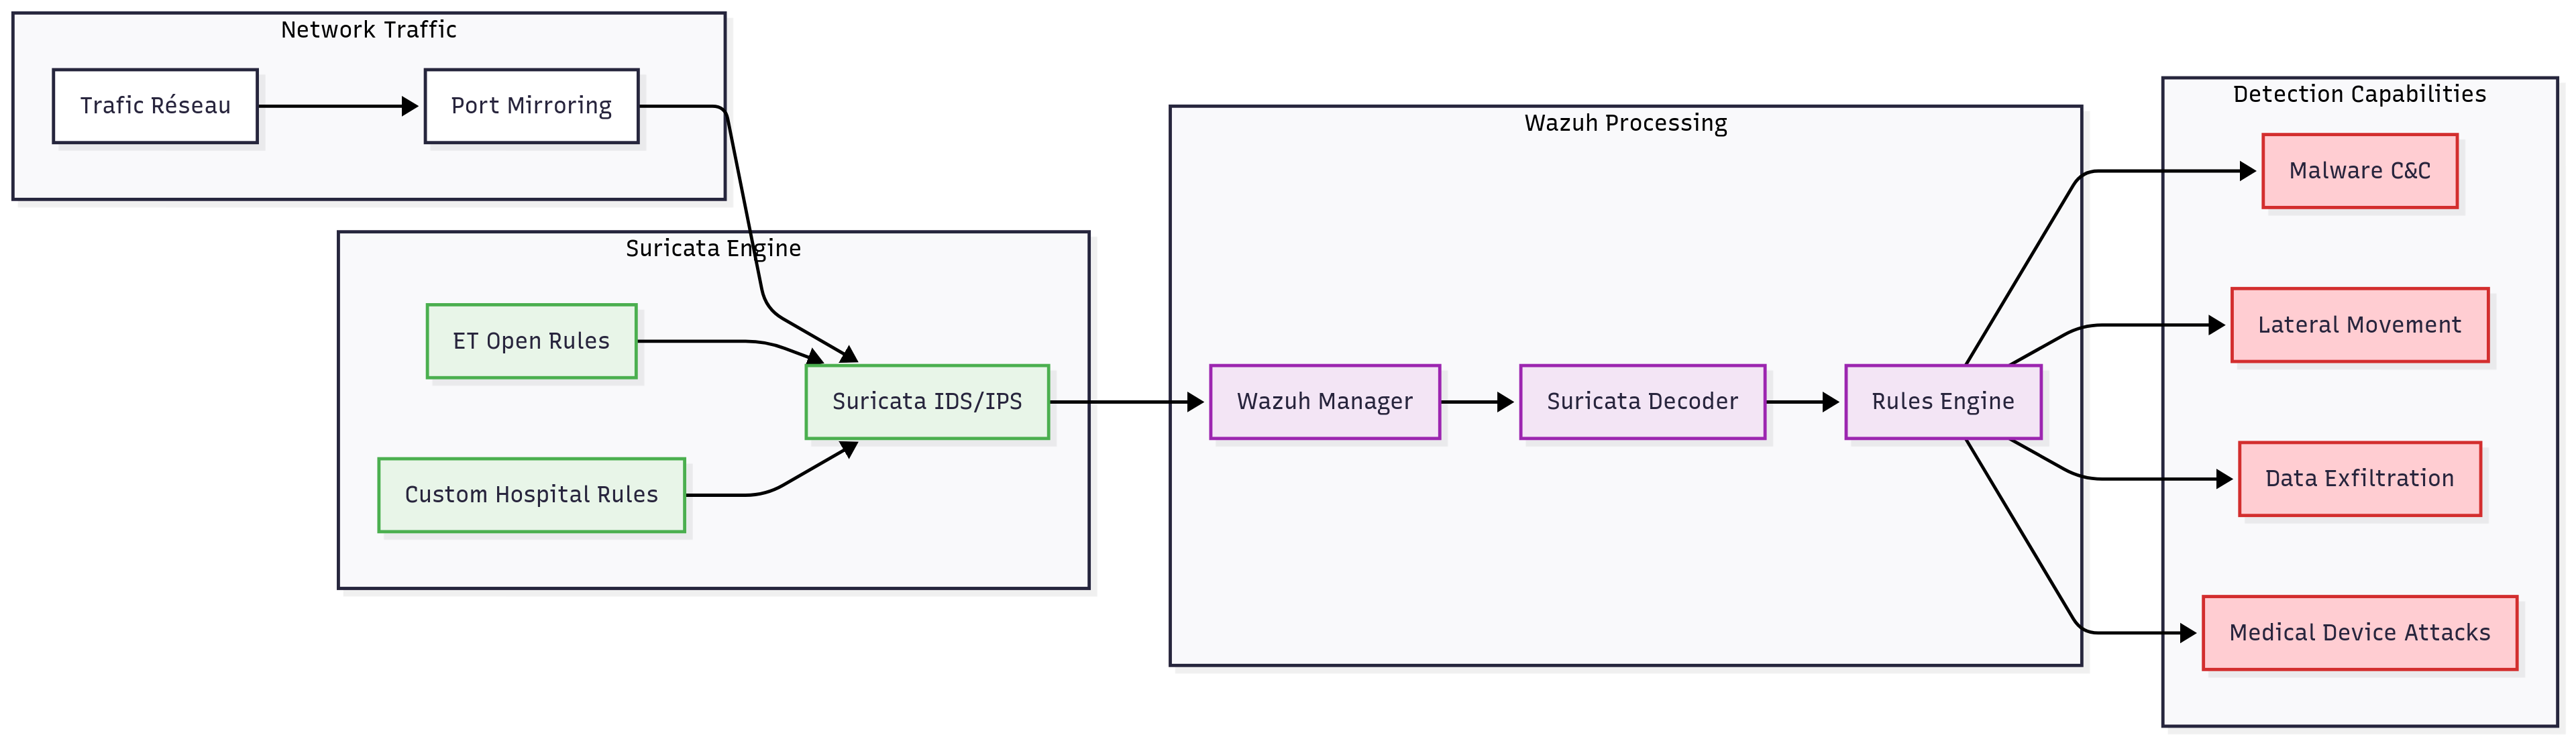
\includegraphics[width=0.9\textwidth]{images/network_security_flow.png}
    \caption{Architecture globale de la solution SIEM/SOAR hospitaliere - Flux de securite}
    \label{fig:architecture_globale}
\end{figure}

La figure \ref{fig:architecture_globale} illustre les flux de donnees et les interactions entre les differents composants de notre solution. Cette architecture garantit une collecte exhaustive des evenements de securite et leur traitement en temps reel.

\subsection{Diagrammes de Flux de Donnees}

\subsubsection{Flux de Donnees Simplifie}

Pour une comprehension initiale, la figure \ref{fig:flow_simple} presente une vue simplifiee des flux de donnees principaux :

\begin{figure}[H]
    \centering
    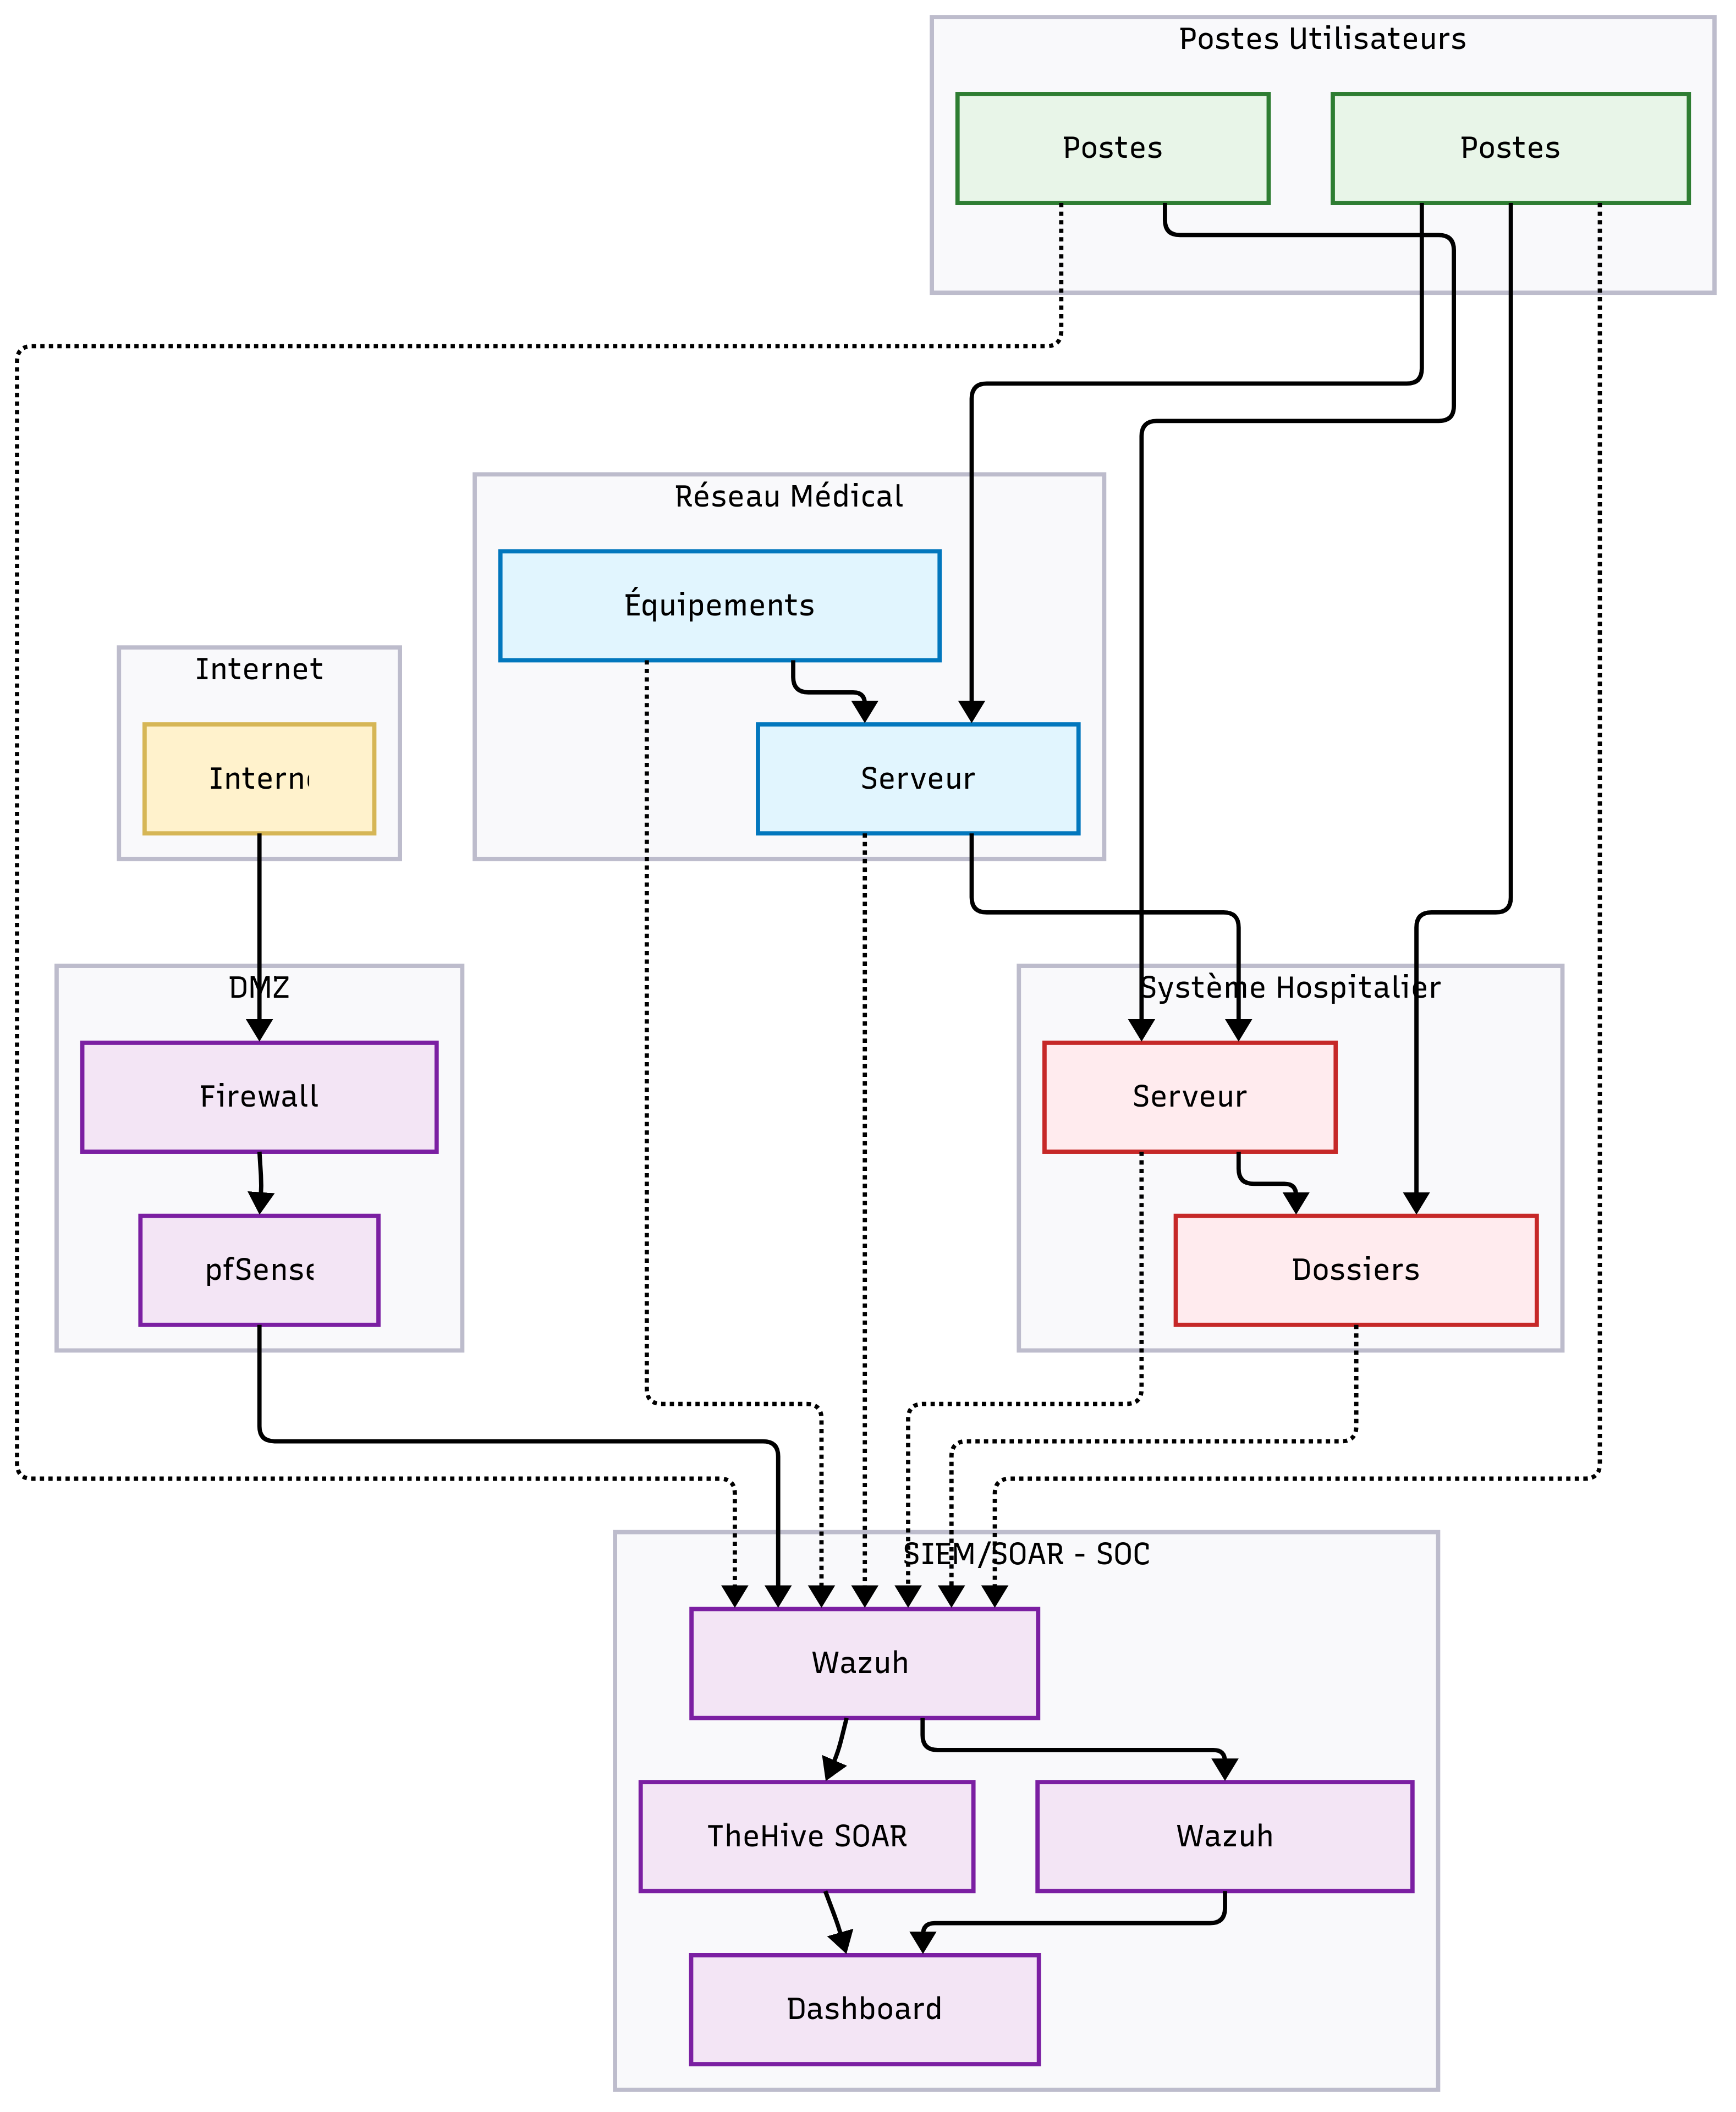
\includegraphics[width=0.8\textwidth]{images/flowData_simple.png}
    \caption{Diagramme de flux de donnees simplifie}
    \label{fig:flow_simple}
\end{figure}

\subsubsection{Couche de Collecte de Donnees}

\paragraph{Sources de Donnees}
\begin{enumerate}
    \item \textbf{Logs Systeme}
          \begin{itemize}
              \item Serveurs Windows ( Sysmon, WazuhAgent)
              \item Serveurs Linux (WazuhAgent)
          \end{itemize}


    \item \textbf{Logs de Securite}
          \begin{itemize}
              \item Firewalls (pfSense)
              \item IDS/IPS (Suricata)
              \item WAF (ModSecurity)
          \end{itemize}

    \item \textbf{Donnees de Contexte}
          \begin{itemize}
              \item Threat Intelligence (MISP feeds)
              \item Vulnerabilites (NIST NVD)
          \end{itemize}
\end{enumerate}

\paragraph{Mecanismes de Collecte}
\begin{itemize}
    \item \textbf{Wazuh Agents} : Deploiement sur endpoints Windows/Linux
    \item \textbf{Syslog forwarding} : Collecte centralisee des logs reseau
    \item \textbf{API REST} : Integration avec applications tierces
    \item \textbf{File monitoring} : Surveillance de fichiers de logs
    \item \textbf{Windows Event Logs} : Collecte native via WinRM
\end{itemize}

\subsection{Couche de Traitement et Correlation}

\subsubsection{Wazuh SIEM - Moteur de Correlation}

\paragraph{Architecture Distribuee}
\begin{itemize}
    \item \textbf{Wazuh Manager} : Serveur central de correlation (Master)
    \item \textbf{Wazuh Workers} : Serveurs de traitement distribue
    \item \textbf{Wazuh Indexer} : Cluster Elasticsearch pour stockage
    \item \textbf{Wazuh Dashboard} : Interface de visualisation Kibana
\end{itemize}

\paragraph{Regles de Correlation Personnalisees}

Les regles de correlation sont developpees pour detecter les attaques specifiques a l'environnement hospitalier :

\begin{lstlisting}[style=xmlstyle,caption=Exemple de regle Wazuh pour detection EternalBlue]
<group name="eternalblue,windows,exploit">
  <!-- EternalBlue SMB exploit detection -->
  <rule id="100001" level="12">
    <if_sid>18152</if_sid>
    <srcip>!$HOME_NET</srcip>
    <dstport>445</dstport>
    <match>SMB|CIFS</match>
    <description>EternalBlue: SMB exploit attempt from external IP</description>
    <group>attack.lateral_movement,attack.t1055</group>
  </rule>
</group>
\end{lstlisting}

\subsubsection{Enrichissement des Evenements}

\paragraph{Geolocalisation IP}
\begin{itemize}
    \item Base GeoIP MaxMind pour localisation geographique
    \item Detection d'acces depuis pays a risque
    \item Calcul de distance impossible (Impossible Travel)
    \item Correlation avec listes de reputation IP
\end{itemize}



\subsection{Couche d'Orchestration SOAR}

\subsubsection{TheHive - Gestion d'Incidents}

\paragraph{Modele de Donnees}
\begin{itemize}
    \item \textbf{Alerts} : Evenements de securite bruts depuis le SIEM
    \item \textbf{Cases} : Incidents de securite confirmes necessitant investigation
    \item \textbf{Tasks} : Actions specifiques dans le cadre d'un incident
    \item \textbf{Observables} : IOCs extraits et analyses (IP, hash, domaine)
\end{itemize}

\paragraph{Workflows Automatises}
\begin{enumerate}
    \item \textbf{Enrichissement Contextuel}
          \begin{itemize}
              \item Recherche historique d'incidents similaires
              \item Correlation avec threat intelligence MISP
          \end{itemize}

    \item \textbf{Reponse Automatisee}
          \begin{itemize}
              \item Isolation reseau d'endpoints compromis
              \item Blocage automatique d'IP malveillantes
              \item Revocation de sessions utilisateur
              \item Sauvegarde forensique de preuves
          \end{itemize}
\end{enumerate}

\subsubsection{Cortex - Analyse d'Observables}

\paragraph{Analyzers Deployes}
\begin{table}[H]
    \centering
    \caption{Analyzers Cortex configures pour l'environnement hospitalier}
    \begin{tabular}{|l|l|c|l|}
        \hline
        \textbf{Type} & \textbf{Analyzer} & \textbf{SLA} & \textbf{Cas d'Usage}    \\
        \hline
        IP            & VirusTotal        & 30s          & Reputation IP externe   \\
        \hline
        URL           & Joe Sandbox       & 5min         & Analyse comportementale \\
        \hline
        Email         & DMARC Analyzer    & 10s          & Validation authenticity \\
        \hline
    \end{tabular}
\end{table}

\paragraph{Responders Personnalises}
\begin{itemize}
    \item \textbf{pfSense IP Block} : Blocage automatique au niveau firewall
    \item \textbf{MISP Event Creation} : Publication IOC vers communaute
\end{itemize}

\subsection{Couche d'Integration et Automatisation}

\subsubsection{n8n - Orchestrateur de Workflows}

\paragraph{Architecture n8n}
\begin{itemize}
    \item \textbf{Execution Mode} : Queue-based avec Redis backend
    \item \textbf{Scaling} : Horizontal scaling avec load balancer
    \item \textbf{Persistence} : PostgreSQL pour etat des workflows
    \item \textbf{Security} : JWT authentication avec rotation automatique
\end{itemize}

\paragraph{Workflows Critiques Implementes}

\begin{enumerate}
    \item \textbf{Workflow EternalBlue Response}
          \begin{itemize}
              \item Trigger : Wazuh alert rule 100001
              \item Actions : Isolation reseau + analyse forensique + notification
              \item SLA : Reponse en < 60 secondes
              \item Escalade : SOC Manager si echec automatisation
          \end{itemize}

    \item \textbf{Workflow XSS Detection}
          \begin{itemize}
              \item Trigger : ModSecurity WAF block
              \item Actions : Analyse payload + bloc IP + notification developpeur
              \item SLA : Traitement en < 30 secondes
          \end{itemize}

    \item \textbf{Workflow Malicious Website}
          \begin{itemize}
              \item Trigger : DNS sinkhole hit
              \item Actions : Investigation utilisateur + formation + rapport
              \item SLA : Investigation en < 24h
              \item Prevention : Mise a jour blacklist DNS
          \end{itemize}
\end{enumerate}

\section{Technologies et Outils Selectionnes}

\subsection{Justification des Choix Techniques}

\subsubsection{Wazuh vs Alternatives}

\begin{table}[H]
    \centering
    \caption{Comparaison des solutions SIEM open source}
    \begin{tabular}{|l|c|c|c|c|}
        \hline
        \textbf{Critere} & \textbf{Wazuh} & \textbf{OSSIM} & \textbf{ELK} & \textbf{Graylog} \\
        \hline
        Events/sec       & 100K+          & 50K            & 200K+        & 75K              \\
        \hline
        Regles natives   & 3000+          & 1500+          & Custom       & 500+             \\
        \hline
        MITRE ATT\&CK    & Natif          & Plugin         & Manual       & Plugin           \\
        \hline
        Agent-based      & Oui            & Oui            & Beats        & Sidecar          \\
        \hline
        File Integrity   & Natif          & Plugin         & Manual       & Plugin           \\
        \hline
        Cloud Ready      & Oui            & Partiel        & Oui          & Oui              \\
        \hline
        \textbf{Score}   & \textbf{9/10}  & 6/10           & 8/10         & 7/10             \\
        \hline
    \end{tabular}
\end{table}

\paragraph{Avantages de Wazuh}
\begin{itemize}
    \item \textbf{Integration native} : MITRE ATT\&CK mapping built-in
    \item \textbf{Performance} : Traitement en temps reel haute performance
    \item \textbf{Compliance} : Modules PCI DSS, HIPAA, SOX natives
    \item \textbf{Scalabilite} : Architecture distribuee avec clustering
    \item \textbf{Communaute} : Support actif et regles regulierement mises a jour
\end{itemize}

\subsubsection{TheHive/Cortex vs Alternatives}

\begin{table}[H]
    \centering
    \caption{Comparaison des plateformes SOAR}
    \begin{tabular}{|l|c|c|c|c|}
        \hline
        \textbf{Critere} & \textbf{TheHive} & \textbf{MISP} & \textbf{Demisto} & \textbf{Phantom} \\
        \hline
        Open Source      & Oui              & Oui           & Non              & Non              \\
        \hline
        API REST         & Complete         & Complete      & Limitee          & Proprietaire     \\
        \hline
        Workflow Engine  & Natif            & Basique       & Avance           & Avance           \\
        \hline
        Threat Intel     & Via MISP         & Natif         & Integre          & Integre          \\
        \hline
        Cost (5 ans)     & 0€               & 0€            & 500K€            & 750K€            \\
        \hline
        Customization    & Elevee           & Elevee        & Moyenne          & Faible           \\
        \hline
        \textbf{Score}   & \textbf{9/10}    & 7/10          & 8/10             & 7/10             \\
        \hline
    \end{tabular}
\end{table}

\subsection{Infrastructure Technique}

\subsubsection{Specifications Materielles}

\begin{table}[H]
    \centering
    \caption{Dimensionnement infrastructure SIEM/SOAR}
    \begin{tabular}{|l|c|c|c|c|}
        \hline
        \textbf{Composant} & \textbf{CPU}     & \textbf{RAM}   & \textbf{Storage} & \textbf{Network} \\
        \hline
        Wazuh Manager      & 4vCPU            & 4 GB           & 5 GB NVMe        & 10 Gbps          \\
        \hline
        Wazuh Indexer      & 2 vCPU           & 2 GB           & 5 GB NVMe        & 10 Gbps          \\
        \hline
        TheHive            & 2 vCPU           & 1 GB           & 5 GB NVMe        & 1 Gbps           \\
        \hline
        Cortex             & 2 vCPU           & 2 GB           & 5 GB NVMe        & 1 Gbps           \\
        \hline
        MISP               & 2 vCPU           & 2 GB           & 5 GB NVMe        & 1 Gbps           \\
        \hline
        n8n                & 2 vCPU           & 3 GB           & 5 GB NVMe        & 1 Gbps           \\
        \hline
        \textbf{Total}     & \textbf{14 vCPU} & \textbf{14 GB} & \textbf{30 GB}   & \textbf{-}       \\
        \hline
    \end{tabular}
\end{table}

\subsubsection{Architecture Reseau}

\paragraph{Segmentation Reseau}
\begin{itemize}
    \item \textbf{WAN} : 192.168.182.0/24 - Interface externe (eth0) vers Internet
    \item \textbf{LAN1} : 192.168.181.0/24 - Segment interne securise (eth2) avec Suricata/WAF
    \item \textbf{LAN2} : 192.168.183.0/24 - Segment test/attaquant (eth1) pour scenarios de penetration
    \item \textbf{HOSPITAL} : 192.168.15.0/24 - Reseau hospitalier principal (SOAR Server, Endpoints)
\end{itemize}


\begin{figure}[H]
    \centering
    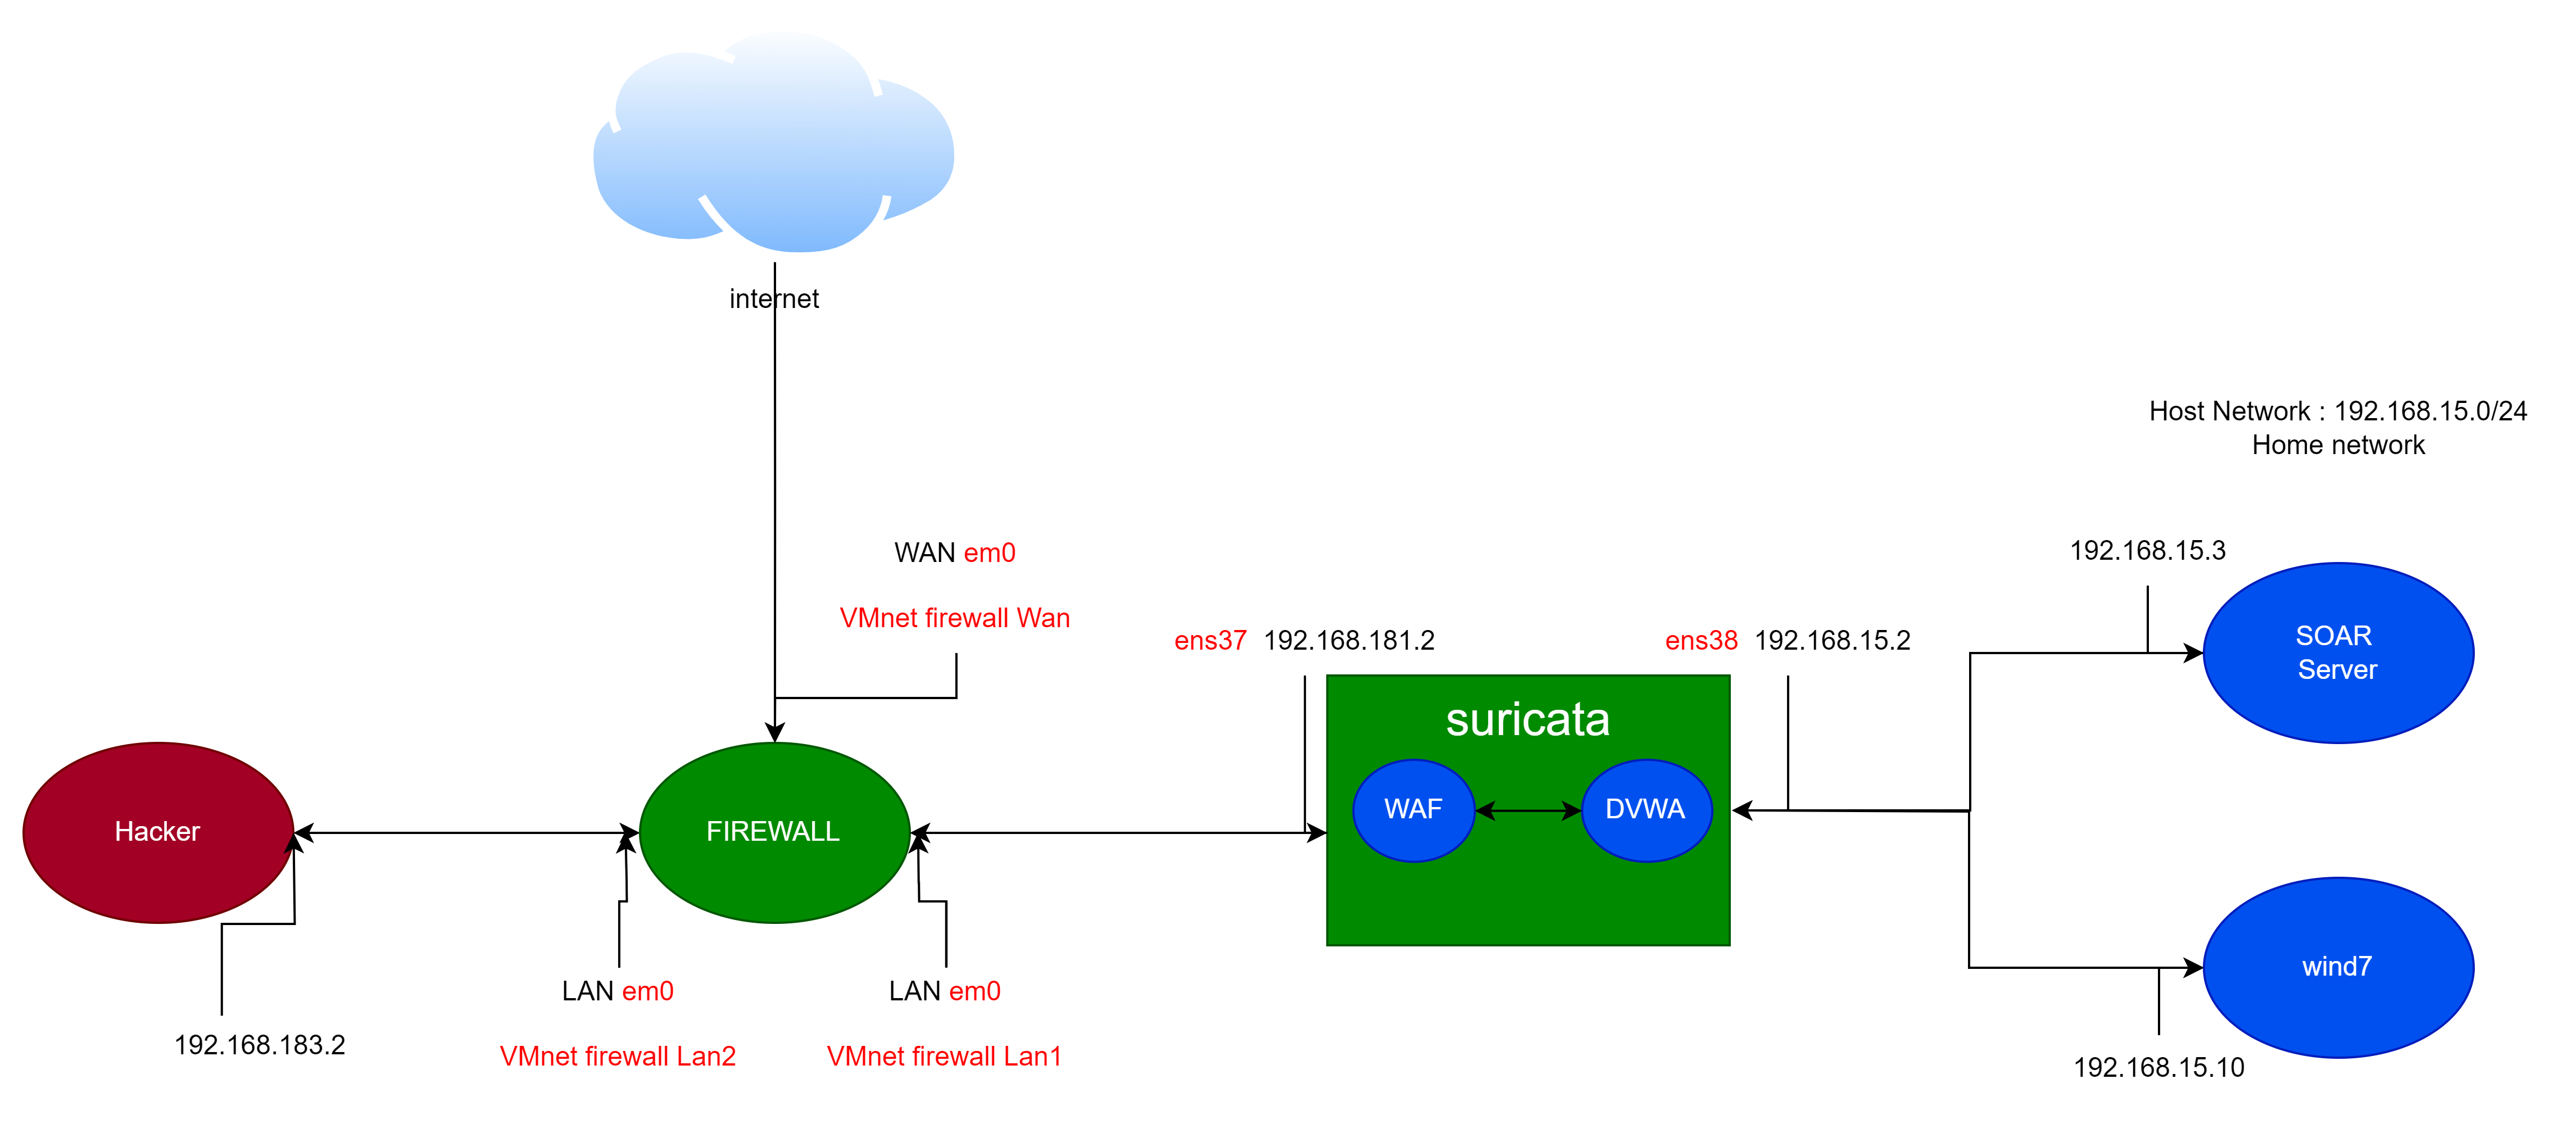
\includegraphics[width=0.8\textwidth]{images/image.png}
    \caption{Topologie reseau hospitaliere - Segmentation et flux autorises}
    \label{fig:topologie_reseau}
\end{figure}

\paragraph{Flux Reseau Autorises}
\begin{enumerate}
    \item HOSPITAL → DMZ SIEM : Syslog (514/UDP), Wazuh Agent (1514/TCP)
    \item DMZ SIEM → LAN SOAR : Elasticsearch (9200/TCP), TheHive API (9000/TCP)
    \item MGMT → All : SSH (22/TCP), SNMP (161/UDP), HTTPS (443/TCP)
\end{enumerate}

Cette approche methodologique et technique etablit les fondements solides pour l'implementation de notre solution SIEM/SOAR, en garantissant la robustesse, la scalabilite et la securite adaptees a l'environnement hospitalier critique.
